\documentclass[tikz,border=12pt]{standalone}
\usepackage{tikz}
\usetikzlibrary{shapes.geometric, positioning, fit, backgrounds, arrows.meta}

\begin{document}
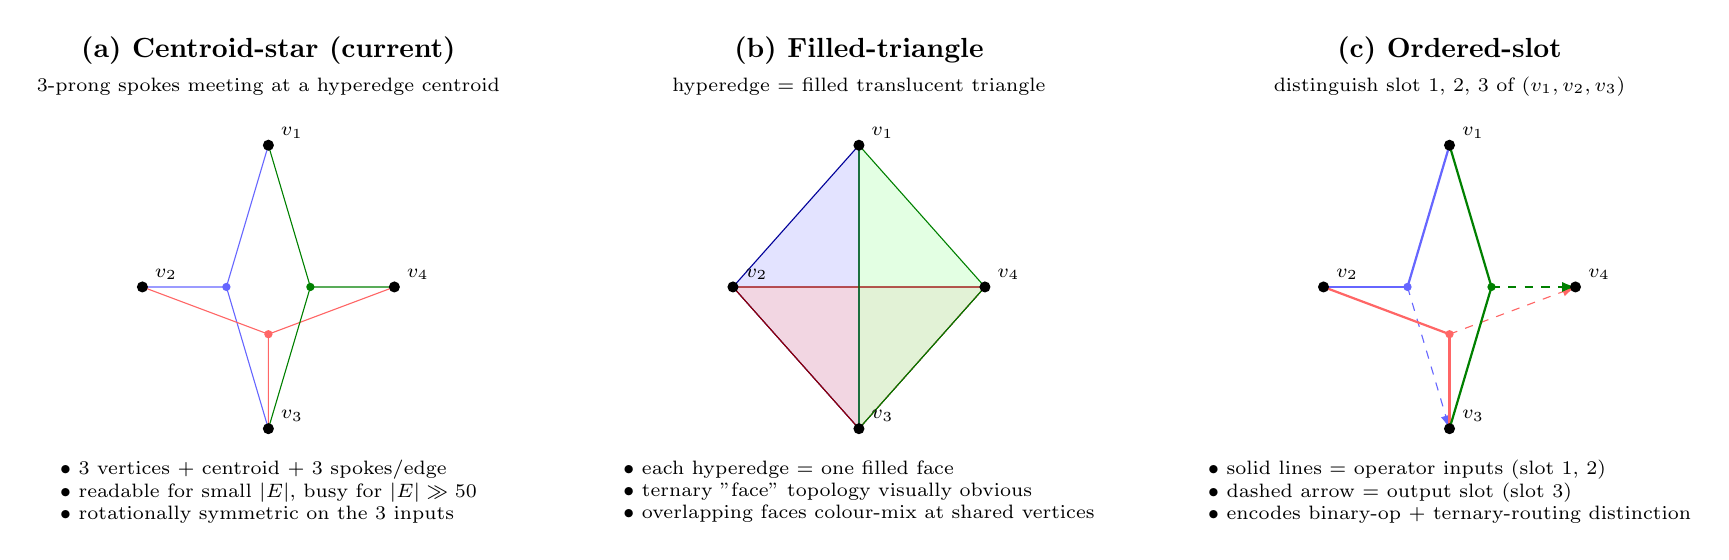
\begin{tikzpicture}[font=\small]

% =============================================================================
% Sample data: a tiny 4-vertex ternary hypergraph with 3 hyperedges
%   e1 = (v1, v2, v3)
%   e2 = (v2, v3, v4)
%   e3 = (v1, v3, v4)
% Same underlying data, three different renderings.
% =============================================================================

% --- Vertex positions (shared across all three panels) ----------------------
% v1 = top, v2 = left, v3 = bottom, v4 = right
% =============================================================================

% ---------- Panel A: current style (centroid-star) ----------
\begin{scope}[shift={(0,0)}]
  \node[font=\bfseries] at (0,3) {(a) Centroid-star (current)};
  \node[font=\scriptsize,align=center] at (0,2.55)
       {3-prong spokes meeting at a hyperedge centroid};

  % Vertices
  \coordinate (v1) at (0, 1.8);
  \coordinate (v2) at (-1.6, 0);
  \coordinate (v3) at (0, -1.8);
  \coordinate (v4) at (1.6, 0);

  % Hyperedge centroids
  \coordinate (e1) at ({(0 + (-1.6) + 0)/3}, {(1.8 + 0 + (-1.8))/3});
  \coordinate (e2) at ({((-1.6) + 0 + 1.6)/3}, {(0 + (-1.8) + 0)/3});
  \coordinate (e3) at ({(0 + 0 + 1.6)/3}, {(1.8 + (-1.8) + 0)/3});

  % Spokes
  \draw[blue!60,thin] (v1)--(e1)--(v2) (e1)--(v3);
  \draw[red!60,thin]  (v2)--(e2)--(v3) (e2)--(v4);
  \draw[green!50!black,thin] (v1)--(e3)--(v3) (e3)--(v4);

  % Centroids
  \fill[blue!60]  (e1) circle (1.5pt);
  \fill[red!60]   (e2) circle (1.5pt);
  \fill[green!50!black] (e3) circle (1.5pt);

  % Vertices
  \foreach \v/\lbl in {v1/$v_1$, v2/$v_2$, v3/$v_3$, v4/$v_4$} {
    \fill[black] (\v) circle (2pt);
    \node[font=\scriptsize, above right=-1pt and 1pt of \v] {\lbl};
  }

  \node[font=\scriptsize, align=left] at (0,-2.6)
    {$\bullet$ 3 vertices + centroid + 3 spokes/edge \\
     $\bullet$ readable for small $|E|$, busy for $|E| \gg 50$ \\
     $\bullet$ rotationally symmetric on the 3 inputs};
\end{scope}

% ---------- Panel B: filled-triangle hyperedge ----------
\begin{scope}[shift={(7.5,0)}]
  \node[font=\bfseries] at (0,3) {(b) Filled-triangle};
  \node[font=\scriptsize,align=center] at (0,2.55)
       {hyperedge = filled translucent triangle};

  \coordinate (v1) at (0, 1.8);
  \coordinate (v2) at (-1.6, 0);
  \coordinate (v3) at (0, -1.8);
  \coordinate (v4) at (1.6, 0);

  % Hyperedge faces (drawn behind vertices, translucent)
  \fill[blue!20,opacity=0.55]  (v1.center)--(v2.center)--(v3.center)--cycle;
  \fill[red!20,opacity=0.55]   (v2.center)--(v3.center)--(v4.center)--cycle;
  \fill[green!20,opacity=0.55] (v1.center)--(v3.center)--(v4.center)--cycle;

  % Boundary outlines (no internal spokes)
  \draw[blue!60!black,thin]  (v1)--(v2)--(v3)--cycle;
  \draw[red!60!black,thin]   (v2)--(v3)--(v4)--cycle;
  \draw[green!50!black,thin] (v1)--(v3)--(v4)--cycle;

  % Vertices
  \foreach \v/\lbl in {v1/$v_1$, v2/$v_2$, v3/$v_3$, v4/$v_4$} {
    \fill[black] (\v) circle (2pt);
    \node[font=\scriptsize, above right=-1pt and 1pt of \v] {\lbl};
  }

  \node[font=\scriptsize, align=left] at (0,-2.6)
    {$\bullet$ each hyperedge = one filled face \\
     $\bullet$ ternary "face" topology visually obvious \\
     $\bullet$ overlapping faces colour-mix at shared vertices};
\end{scope}

% ---------- Panel C: ordered-slot rendering ----------
\begin{scope}[shift={(15,0)}]
  \node[font=\bfseries] at (0,3) {(c) Ordered-slot};
  \node[font=\scriptsize,align=center] at (0,2.55)
       {distinguish slot 1, 2, 3 of $(v_1, v_2, v_3)$};

  \coordinate (v1) at (0, 1.8);
  \coordinate (v2) at (-1.6, 0);
  \coordinate (v3) at (0, -1.8);
  \coordinate (v4) at (1.6, 0);

  % Hyperedge "node" — labeled centroid with arrow into slot 3
  \coordinate (e1) at ({(0 + (-1.6) + 0)/3}, {(1.8 + 0 + (-1.8))/3});
  \coordinate (e2) at ({((-1.6) + 0 + 1.6)/3}, {(0 + (-1.8) + 0)/3});
  \coordinate (e3) at ({(0 + 0 + 1.6)/3}, {(1.8 + (-1.8) + 0)/3});

  % e1 = (v1, v2, v3): solid lines from v1,v2 (operator inputs); dashed to v3 (output slot)
  \draw[blue!60,thick] (v1)--(e1);
  \draw[blue!60,thick] (v2)--(e1);
  \draw[blue!60,dashed,-{Latex}] (e1)--(v3);

  % e2 = (v2, v3, v4)
  \draw[red!60,thick] (v2)--(e2);
  \draw[red!60,thick] (v3)--(e2);
  \draw[red!60,dashed,-{Latex}] (e2)--(v4);

  % e3 = (v1, v3, v4)
  \draw[green!50!black,thick] (v1)--(e3);
  \draw[green!50!black,thick] (v3)--(e3);
  \draw[green!50!black,dashed,-{Latex}] (e3)--(v4);

  \fill[blue!60]  (e1) circle (1.5pt);
  \fill[red!60]   (e2) circle (1.5pt);
  \fill[green!50!black] (e3) circle (1.5pt);

  \foreach \v/\lbl in {v1/$v_1$, v2/$v_2$, v3/$v_3$, v4/$v_4$} {
    \fill[black] (\v) circle (2pt);
    \node[font=\scriptsize, above right=-1pt and 1pt of \v] {\lbl};
  }

  \node[font=\scriptsize, align=left] at (0,-2.6)
    {$\bullet$ solid lines = operator inputs (slot 1, 2) \\
     $\bullet$ dashed arrow = output slot (slot 3) \\
     $\bullet$ encodes binary-op + ternary-routing distinction};
\end{scope}

\end{tikzpicture}
\end{document}
